\documentclass[a4paper,12pt]{article}
\usepackage{standalone}
\usepackage[a4paper, top=0.8in, bottom=0.7in, left=0.8in, right=0.8in]{geometry}
\usepackage{amsmath}
\usepackage{hyperref}
\usepackage{amsfonts}
\usepackage{latexsym}
\usepackage{graphicx}
\usepackage{fancyhdr}
\usepackage{enumitem}
\usepackage{setspace}
\usepackage{tcolorbox}
\usepackage{tikz}
\usepackage{multicol}
\usepackage{xcolor}
\usepackage[defaultfam,tabular,lining]{montserrat} % Font settings for Montserrat

% Hyperref settings for colored and clickable links
\hypersetup{
    colorlinks=true,
    linkcolor=blue,
    urlcolor=blue,
    filecolor=blue,
    menucolor=blue,
}

\sloppy

\title{}
\date{}
\hyphenpenalty=10000
\exhyphenpenalty=10000

\setlength{\parindent}{0pt}
\pagestyle{fancy}

\setlength{\headheight}{27.11148pt}
\addtolength{\topmargin}{-15.11148pt}

% Change these commands to update throughout the document
\newcommand{\standards}{CCSS}    % Standard Set (e.g., CCSS, Georgia)
\newcommand{\subject}{Math}      % Subject Name
\newcommand{\levelLetter}{H}     % Curriculum Level (Grade 7)
\newcommand{\doctype}{SWB}       % Document Type (SWB, TWB, etc.)

% Document Title Command
\newcommand{\doctitle}{\standards\ \subject\ Curriculum \levelLetter\ \doctype}

\fancyhf{}
\fancyhead[L]{\textbf{\doctitle}}
\fancyhead[R]{
\includegraphics[width=0.8cm]{Round Logo.png}} % Placeholder for logo
\fancyfoot[C]{\footnotesize \textcopyright{} Study Smart Tutors}
\fancyfoot[R]{\thepage}  % Page number in bottom right corner
\fancyfoot[L]{\hyperlink{toc}{Back to Contents}} % Clickable link in bottom left to TOC

% Reset page numbers after TOC
\newcommand{\startPageNumbers}{\setcounter{page}{1}}

\sloppy

%%%%%%%%%%%%%%%%%%%%%%%%%%%%%%%%%%%%%

\begin{document}

% Title Page
\documentclass[12pt]{article}
\usepackage[a4paper, top=0.8in, bottom=0.7in, left=0.8in, right=0.8in]{geometry}
\usepackage{amsmath}
\usepackage{amsfonts}
\usepackage{latexsym}
\usepackage{graphicx}
\usepackage{tikz}
\usepackage{fancyhdr}
\usepackage{tcolorbox}
\usepackage{multicol}
\usepackage{tgadventor}
\renewcommand{\familydefault}{\sfdefault}
\usepackage{enumitem}
\usepackage{setspace}
\setlength{\parindent}{0pt}
\pagestyle{fancy}
\usepackage{needspace}


% Define a new command for the level letter
\newcommand{\levelLetter}{H}  % Change this letter to update throughout the document

%%%%%%%%%%%%%%%%%%%%%%%%%%%%%%%%%%%%%

\setlength{\headheight}{27.11148pt}
\addtolength{\topmargin}{-15.11148pt}

\fancyhf{}
%\fancyhead[L]{\textbf{5.NBT.A.1: Understand the Place Value System}}
\fancyhead[R]{
\includegraphics[width=0.8cm]{Round Logo.png}}
\fancyfoot[C]{\footnotesize © Study Smart Tutors}






\title{}
\date{}
\hyphenpenalty=10000
\exhyphenpenalty=10000

\begin{document}


% COVER PAGE 1 BEGIN
% Skip header and footer on the first page
\thispagestyle{empty}

% Vertical centering
\vspace*{\fill}

\vspace*{3cm}

\begin{center}

    % Logo
    
\includegraphics[width=0.6\textwidth]{SST_Color_Logo.png} % Replace 'logo.png' with the path to your logo file
    
    \vspace{1cm} % Space between logo and title
    
    % Cycle Name
    \Huge \textbf{} \\
    \vspace{0.2cm}
    
    % Assessment Title
    \Huge \textbf{Mathematics Tutoring}\\ 
     \vspace{1 cm}
      \LARGE \textit{Curriculum \levelLetter}\\[1cm]
 \vspace{0.5cm}
    
   


     % Name Field
    \LARGE \textbf{Name:} \underline{\hspace{8cm}}

    
    \vfill % Push the footer to the bottom
    
\end{center}


\newpage
\thispagestyle{empty}
\vspace*{\fill}
\newpage


\newpage


% STUDENT COVER PAGE  COMPLETE


\end{document}


% Table of Contents
\pagenumbering{gobble}
\hypertarget{toc}{}
\tableofcontents
\newpage
\startPageNumbers

% Restart page numbering from 1 after TOC
\pagenumbering{arabic}
\pagestyle{fancy}  % Re-enable fancy headers/footers

% Guided Lesson and Problem Set for 7.RP.A.2a, 7.RP.A.2b
\newpage
\section{7.RP.A.2a, 7.RP.A.2b Guided Lesson}
\documentclass[12pt]{article}
\usepackage[a4paper, top=0.8in, bottom=0.7in, left=0.8in, right=0.8in]{geometry}
\usepackage{amsmath}
\usepackage{amsfonts}
\usepackage{latexsym}
\usepackage{graphicx}
\usepackage{fancyhdr}
\usepackage{enumitem}
\usepackage{setspace}
\usepackage{tcolorbox}
\usepackage{textcomp}
\usepackage[defaultfam,tabular,lining]{montserrat}

% General Comment: Template for creating guided lessons in a structured format with headers, titles, and sections.

\setlength{\parindent}{0pt}
\pagestyle{fancy}

\setlength{\headheight}{27.11148pt}
\addtolength{\topmargin}{-15.11148pt}

\fancyhf{}
%\fancyhead[L]{\textbf{Standard(s): 7.RP.A.2a, 7.RP.A.2b}}
\fancyhead[R]{
\includegraphics[width=0.8cm]{Round Logo.png}}
\fancyfoot[C]{\footnotesize © Study Smart Tutors}

\sloppy

\title{}
\date{}
\hyphenpenalty=10000
\exhyphenpenalty=10000

\begin{document}

\subsection*{Guided Lesson: Recognizing and Representing Proportional Relationships}
\onehalfspacing

% Learning Objective Box
\begin{tcolorbox}[colframe=black!40, colback=gray!5, 
coltitle=black, colbacktitle=black!20, fonttitle=\bfseries\Large, 
title=Learning Objective, halign title=center, left=5pt, right=5pt, top=5pt, bottom=15pt]
\textbf{Objective:} Understand and identify proportional relationships using tables, graphs, and equations. Represent these relationships to solve real-world problems.
\end{tcolorbox}

\vspace{1em}

% Key Concepts and Vocabulary
\begin{tcolorbox}[colframe=black!60, colback=white, 
coltitle=black, colbacktitle=black!15, fonttitle=\bfseries\Large, 
title=Key Concepts and Vocabulary, halign title=center, left=10pt, right=10pt, top=10pt, bottom=15pt]
\textbf{Key Concepts:}
\begin{itemize}
    \item \textbf{Proportional Relationships:} A relationship between two quantities is proportional if they increase or decrease at the same rate. 
    \item \textbf{Constant of Proportionality (Unit Rate):} The constant ratio between two proportional quantities, often represented as \(k\). For example, if \( y = kx \), then \(k = \frac{y}{x}\).
    \item \textbf{Graphs:} A graph represents a proportional relationship if it is a straight line passing through the origin.
    \item \textbf{Equations:} Proportional relationships can be written in the form \(y = kx\), where \(k\) is the constant of proportionality.
\end{itemize}
\end{tcolorbox}

\vspace{1em}

% Examples
\begin{tcolorbox}[colframe=black!60, colback=white, 
coltitle=black, colbacktitle=black!15, fonttitle=\bfseries\Large, 
title=Examples, halign title=center, left=10pt, right=10pt, top=10pt, bottom=15pt]
\textbf{Example 1: Proportional Relationship in a Table}
\begin{itemize}
    \item Problem: A car travels at a constant speed. The table shows the relationship between the time (\(x\)) in hours and the distance (\(y\)) in miles:
    \[
    \begin{array}{|c|c|}
    \hline
    \text{Time (hours)} & \text{Distance (miles)} \\
    \hline
    1 & 60 \\
    2 & 120 \\
    3 & 180 \\
    \hline
    \end{array}
    \]
    \item Solution: Find the constant ratio \(k = \frac{y}{x}\). For each row, \( \frac{60}{1} = 60 \), \( \frac{120}{2} = 60 \), \( \frac{180}{3} = 60 \). The constant of proportionality is \(k = 60\). The equation is \(y = 60x\).
\end{itemize}

\textbf{Example 2: Proportional Relationship in a Graph}
\begin{itemize}
    \item Problem: The graph below represents the relationship between the number of gallons of gas purchased and the total cost:
    

    \item Solution: The graph is a straight line passing through the origin, so the relationship is proportional. The constant of proportionality is the slope of the line. From the graph, \(k = \frac{\text{Cost}}{\text{Gallons}} = 3\). The equation is \(y = 3x\).
\end{itemize}

\textbf{Example 3: Writing an Equation}
\begin{itemize}
    \item Problem: A recipe requires 2 cups of sugar for every 5 cups of flour. Write an equation to represent the relationship.
    \item Solution: The constant of proportionality is \(k = \frac{2}{5}\). The equation is \(y = \frac{2}{5}x\), where \(x\) is the number of cups of flour, and \(y\) is the number of cups of sugar.
\end{itemize}
\end{tcolorbox}

\vspace{1em}

% Guided Practice
\begin{tcolorbox}[colframe=black!60, colback=white, 
coltitle=black, colbacktitle=black!15, fonttitle=\bfseries\Large, 
title=Guided Practice, halign title=center, left=10pt, right=10pt, top=10pt, bottom=15pt]
\textbf{Solve the following problems with teacher support:}
\begin{enumerate}[itemsep=5em]
    \item The table below shows the relationship between hours worked (\(x\)) and money earned (\(y\)):
    \[
    \begin{array}{|c|c|}
    \hline
    \text{Hours Worked} & \text{Money Earned} \\
    \hline
    2 & 30 \\
    4 & 60 \\
    6 & 90 \\
    \hline
    \end{array}
    \]
    Determine the constant of proportionality and write the equation.
    \item A proportional relationship is represented by the equation \(y = 4x\). Create a table and graph the relationship.
    \item A store sells 3 pounds of apples for \$9. Write an equation to represent the cost of \(x\) pounds of apples. What is the cost of 7 pounds?
\end{enumerate}
\end{tcolorbox}

\vspace{1em}

% Additional Notes
\begin{tcolorbox}[colframe=black!40, colback=gray!5, 
coltitle=black, colbacktitle=black!20, fonttitle=\bfseries\Large, 
title=Additional Notes, halign title=center, left=5pt, right=5pt, top=5pt, bottom=15pt]
\textbf{Helpful Tips:}
\begin{itemize}
    \item A graph of a proportional relationship always passes through the origin.
    \item The constant of proportionality can be found using the equation \(k = \frac{y}{x}\).
    \item When writing equations, clearly define the variables.
\end{itemize}
\end{tcolorbox}

\vspace{1em}

% Independent Practice
\begin{tcolorbox}[colframe=black!60, colback=white, 
coltitle=black, colbacktitle=black!15, fonttitle=\bfseries\Large, 
title=Independent Practice, halign title=center, left=10pt, right=10pt, top=10pt, bottom=15pt]
\textbf{Solve the following problems independently:}
\begin{enumerate}[itemsep=5em]
    \item A car travels 50 miles for every gallon of gas. Write an equation to represent the relationship and use it to find the distance traveled on 8 gallons of gas.
    \item The table below shows a proportional relationship. Find the constant of proportionality and write the equation:
    \[
    \begin{array}{|c|c|}
    \hline
    \text{Minutes} & \text{Pages Read} \\
    \hline
    10 & 20 \\
    15 & 30 \\
    25 & 50 \\
    \hline
    \end{array}
    \]
    \item A graph passes through the points \((0, 0)\) and \((5, 15)\). Write the equation of the proportional relationship.
\end{enumerate}
\end{tcolorbox}

\vspace{1em}

% Exit Ticket
\begin{tcolorbox}[colframe=black!60, colback=white, 
coltitle=black, colbacktitle=black!15, fonttitle=\bfseries\Large, 
title=Exit Ticket, halign title=center, left=10pt, right=10pt, top=10pt, bottom=15pt]
\textbf{Reflect and solve:}
\begin{itemize}
    \item How can you identify a proportional relationship in a graph, table, or equation? Provide an example for each.
\end{itemize}
\end{tcolorbox}

\end{document}


\newpage
\section{7.RP.A.2a, 7.RP.A.2b Problem Set}
% ChatGPT Directions 0 :
% This is a Tbox Problem set for the following standards 7.RP.A.2a, 7.RP.A.2b
%--------------------------------------------------
\documentclass[12pt]{article}
\usepackage[a4paper, top=0.8in, bottom=0.7in, left=0.8in, right=0.8in]{geometry}
\usepackage{amsmath}
\usepackage{amsfonts}
\usepackage{latexsym}
\usepackage{graphicx}
\usepackage{fancyhdr}
\usepackage{tcolorbox}
\usepackage{enumitem}
\usepackage{setspace}
\usepackage{pgfplots}
\usepackage{tikz}
\usepackage[defaultfam,tabular,lining]{montserrat} % Font settings for Montserrat

% General Comment: Template for creating problem sets in a structured format with headers, titles, and sections.
% This document uses Montserrat font and consistent styles for exercises, problems, and performance tasks.

% -------------------------------------------------------------------

%    - Include a header with standards and topic title: \fancyhead[L]{\textbf{<Standards>: <Topic Title>}}.
%    - Use "Problem Set:" as the prefix for subsection titles, followed by the topic title.
%    - Example: \subsection*{Problem Set: Understanding Multiplication and Division}.
%
% 2. **Section Breakdown**:
%    - **Learning Objective**: A concise statement summarizing the goal of the problem set.
%    - **Exercises**: Focus on procedural fluency with straightforward tasks.
%    - **Problems**: Include moderately complex scenarios requiring reasoning or application.
%    - **Performance Task**: Real-world, open-ended tasks that require multi-step solutions or creative thinking.
%    - **Reflection**: Prompt students to reflect on their strategies and learning.
%
% 3. **Styling with tcolorbox**:
%    - Use the following guidelines for tcolorbox styling:
%        - **Frame color**: black or dark gray (colframe=black!60).
%        - **Background color**: light gray or white (colback=gray!5 or colback=white).
%        - **Title background**: slightly darker gray (colbacktitle=black!15).
%        - **Font style**: Bold and large for titles (fonttitle=\bfseries\Large).
%
% 4. **Content and Alignment**:
%    - Align tasks with the defined standard(s).
%    - Ensure a balance of exercises (procedural), problems (conceptual), and performance tasks (application).
%    - Adjust spacing for student work using `\vspace` and `itemsep` as needed.
%
% 5. **Definitions**:
%    - **Exercises**: Develop fluency (e.g., basic computations or simple tasks).
%    - **Problems**: Build understanding with moderately complex applications.
%    - **Performance Tasks**: Require real-world application, design, or explanation.
%
% 6. **Example**:
%    - For an exercise: "Find the quotient of \(56 \div 8\)."
%    - For a problem: "A recipe calls for \(2/3\) of a cup of sugar. How much sugar is needed for \(3\) batches?"
%    - For a performance task: "Design a seating arrangement for a classroom using fractions to represent groups."
% -------------------------------------------------------------------

\setlength{\parindent}{0pt}
\pagestyle{fancy}

\setlength{\headheight}{27.11148pt}
\addtolength{\topmargin}{-15.11148pt}

\fancyhf{}
%\fancyhead[L]{\textbf{7.RP.A.2a, 7.RP.A.2b: Understanding Proportional Relationships}}
\fancyhead[R]{
\includegraphics[width=0.8cm]{Round Logo.png}} % Placeholder for logo
\fancyfoot[C]{\footnotesize © Study Smart Tutors}

\sloppy

\title{}
\date{}
\hyphenpenalty=10000
\exhyphenpenalty=10000

\newcommand{\dfrac}[2]{\dfrac{#1}{#2}} % New command for display style fractions
\pgfplotsset{compat=1.18} 


\begin{document}

\subsection*{Problem Set: Understanding Proportional Relationships}
\onehalfspacing

% Learning Objective Box
\begin{tcolorbox}[colframe=black!40, colback=gray!5, 
coltitle=black, colbacktitle=black!20, fonttitle=\bfseries\Large, 
title=Learning Objective, halign title=center, left=5pt, right=5pt, top=5pt, bottom=15pt]
\textbf{Objective:} Solve problems involving proportional relationships and represent these relationships using equations with variables.
\end{tcolorbox}

% Exercises Box
\begin{tcolorbox}[colframe=black!60, colback=white, 
coltitle=black, colbacktitle=black!15, fonttitle=\bfseries\Large, 
title=Exercises, halign title=center, left=10pt, right=10pt, top=10pt, bottom=35pt]
\begin{enumerate}[itemsep=2em]
    \item Find the unit rate: \( \dfrac{84}{7} \).
    \item Write an equation for the relationship: "If 3 apples cost \$6, how much will \(x\) apples cost?"
    \item Solve: \(4x = 48\).
    \item Complete the table for the proportional relationship:
    \newline 
    \begin{tabular}{|c|c|}
        \hline
        Number of Items & Cost (in \$) \\ \hline
        2 & 10 \\ \hline
        5 & \_\_\_ \\ \hline
        8 & \_\_\_ \\ \hline
    \end{tabular}
    \item A machine produces 120 widgets in 4 hours. Find the rate of production (widgets per hour).
    \item Determine if the following table represents a proportional relationship.  If yes, write the equation. If not, explain why not. \\
    \newline
    \begin{tabular}{|c|c|}
        \hline
        \(x\) & \(y\) \\ \hline
        1 & 3 \\ \hline
        2 & 6 \\ \hline
        3 & 9 \\ \hline
        4 & 11 \\ \hline
    \end{tabular}
   
    \item If \(y\) is proportional to \(x\), and \(y = 24\) when \(x = 6\), find the constant of proportionality \(k\). Write the equation.

\end{enumerate}
\end{tcolorbox}

\vspace{1em}

% Problems Box
\begin{tcolorbox}[colframe=black!60, colback=white, 
coltitle=black, colbacktitle=black!15, fonttitle=\bfseries\Large, 
title=Problems, halign title=center, left=10pt, right=10pt, top=10pt, bottom=30pt]
\begin{enumerate}[start=9, itemsep=3em]
    \item A car travels 180 miles in 3 hours. 
    \begin{enumerate}[label=(\alph*)]
        \item Find the speed of the car (miles per hour).  
        \item Write an equation for the total distance \(d\) as a function of time \(t\).  
    \end{enumerate}
    \item A store sells 4 bags of rice for \$20.  
    \begin{enumerate}[label=(\alph*)]
        \item Write an equation for the total cost \(C\) as a function of the number of bags \(x\).  
        \item Determine the cost for 7 bags of rice.  
    \end{enumerate}
    \item A recipe uses 3 cups of flour to make 6 servings.  
    \begin{enumerate}[label=(\alph*)]
        \item Find the constant of proportionality.  
        \item How many cups of flour are needed to make 12 servings?  
    \end{enumerate}
        \item Graph the proportional relationship represented by the equation \(y = 3x\).
         
    \begin{center}
\begin{tikzpicture}[scale=0.8]
    \draw[thick,->] (0,0) -- (11,0) node[right]{\(x\)};
    \draw[thick,->] (0,0) -- (0,11) node[above]{\(y\)};

    % Add grid lines
    \foreach \x in {1,...,10} {
        \draw[gray, thin] (\x,0) -- (\x,11);
    }
    \foreach \y in {1,...,10} {
        \draw[gray, thin] (0,\y) -- (11,\y);
    }

    \foreach \x in {0,1,...,10} {
        \draw (\x,0.1) -- (\x,-0.1) node[below]{\x};
    }
    \foreach \y in {0,1,...,10} {
        \draw (0.1,\y) -- (-0.1,\y) node[left]{\y};
    }
\end{tikzpicture}
\end{center}
    % \item Graph the proportional relationship represented by the table below:
    % \newline
    % \begin{tabular}{|c|c|}
    %     \hline
    %     \(x\) & \(y\) \\ \hline
    %     1 & 2 \\ \hline
    %     2 & 4 \\ \hline
    %     3 & 6 \\ \hline
    %     4 & 8 \\ \hline
    % \end{tabular}


    
\end{enumerate}
\end{tcolorbox}

% Performance Task Box
\vspace{1em}
\begin{tcolorbox}[colframe=black!60, colback=white, 
coltitle=black, colbacktitle=black!15, fonttitle=\bfseries\Large, 
title=Performance Task: Planning a Shopping Trip, halign title=center, left=10pt, right=10pt, top=10pt, bottom=80pt]
You are shopping for school supplies. Here’s what you know:
\begin{itemize}
    \item Notebooks cost \$3 each.
    \item Pencils are \$0.50 each.
    \item You have a budget of \$30.
\end{itemize}
\textbf{Task:}
\begin{enumerate}[itemsep=4em]
    \item Write an equation to represent the total cost of buying \(n\) notebooks and \(p\) pencils.
    \item Determine how many notebooks and pencils you can buy if you spend exactly \$30.
    \item Design a plan to maximize the number of items purchased while staying within budget.
\end{enumerate}
\end{tcolorbox}

% Reflection Box
\vspace{1em}
\begin{tcolorbox}[colframe=black!60, colback=white, 
coltitle=black, colbacktitle=black!15, fonttitle=\bfseries\Large, 
title=Reflection, halign title=center, left=10pt, right=10pt, top=10pt, bottom=110pt]
What strategies did you use to solve the performance task? How does identifying proportional relationships help in solving real-world problems? Share any patterns or observations.
\end{tcolorbox}

\end{document}


% Guided Lesson and Problem Set for 7.RP.A.3
\newpage
\section{7.RP.A.3 Guided Lesson}
\documentclass[12pt]{article}
\usepackage[a4paper, top=0.8in, bottom=0.7in, left=0.8in, right=0.8in]{geometry}
\usepackage{amsmath}
\usepackage{amsfonts}
\usepackage{latexsym}
\usepackage{graphicx}
\usepackage{fancyhdr}
\usepackage{enumitem}
\usepackage{setspace}
\usepackage{tcolorbox}
\usepackage{textcomp}
\usepackage[defaultfam,tabular,lining]{montserrat}

% General Comment: Template for creating guided lessons in a structured format with headers, titles, and sections.

\setlength{\parindent}{0pt}
\pagestyle{fancy}

\setlength{\headheight}{27.11148pt}
\addtolength{\topmargin}{-15.11148pt}

\fancyhf{}
%\fancyhead[L]{\textbf{Standard(s): 7.RP.A.3}}
\fancyhead[R]{
\includegraphics[width=0.8cm]{Round Logo.png}}
\fancyfoot[C]{\footnotesize © Study Smart Tutors}

\sloppy

\title{}
\date{}
\hyphenpenalty=10000
\exhyphenpenalty=10000

\begin{document}

\subsection*{Guided Lesson: Solving Multi-Step Proportional Problems with Percentages}
\onehalfspacing

% Learning Objective Box
\begin{tcolorbox}[colframe=black!40, colback=gray!5, 
coltitle=black, colbacktitle=black!20, fonttitle=\bfseries\Large, 
title=Learning Objective, halign title=center, left=5pt, right=5pt, top=5pt, bottom=15pt]
\textbf{Objective:} Solve multi-step proportional problems involving percentages such as tax, tips, discounts, and multi-part cost problems using equations, proportions, and logical reasoning.
\end{tcolorbox}

\vspace{1em}

% Key Concepts and Vocabulary
\begin{tcolorbox}[colframe=black!60, colback=white, 
coltitle=black, colbacktitle=black!15, fonttitle=\bfseries\Large, 
title=Key Concepts and Vocabulary, halign title=center, left=10pt, right=10pt, top=10pt, bottom=15pt]
\textbf{Key Concepts:}
\begin{itemize}
    \item \textbf{Proportional Relationships:} Use proportions to relate parts and wholes in percentage problems. For example:
    \[
    \frac{\text{Part}}{\text{Whole}} = \frac{\text{Percent}}{100}.
    \]
    \item \textbf{Percent Calculations:}
    \begin{itemize}
        \item \textbf{Tax and Tip:} Add the calculated percentage to the original amount.
        \item \textbf{Discounts:} Subtract the calculated percentage from the original amount.
        \item \textbf{Multi-Step Problems:} When combining multiple steps (e.g., applying a discount and then adding tax), solve one step at a time.
    \end{itemize}
    \item \textbf{Percent Equation:} Use the equation \(\text{Part} = \text{Percent} \times \text{Whole}\) to find missing values.
    \item \textbf{Unit Rates:} Calculate cost per unit by dividing the total cost by the quantity to solve proportional pricing problems.
\end{itemize}
\end{tcolorbox}

\vspace{1em}

% Examples
\begin{tcolorbox}[colframe=black!60, colback=white, 
coltitle=black, colbacktitle=black!15, fonttitle=\bfseries\Large, 
title=Examples, halign title=center, left=10pt, right=10pt, top=10pt, bottom=15pt]
\textbf{Example 1: Calculating Tax and Total Cost}
\begin{itemize}
    \item Problem: A jacket costs \$80, and the sales tax is 9\%. What is the total cost, including tax?
    \item Solution:
    \begin{itemize}
        \item Step 1: Calculate the tax: \( 80 \times 0.09 = 7.20 \).
        \item Step 2: Add the tax to the original cost: \( 80 + 7.20 = 87.20 \).
        \item Final Answer: The total cost is \$87.20.
    \end{itemize}
\end{itemize}

\textbf{Example 2: Solving a Multi-Step Problem}
\begin{itemize}
    \item Problem: A television is originally \$500. It is on sale for 20\% off, and there is an additional \$25 rebate. What is the final price?
    \item Solution:
    \begin{itemize}
        \item Step 1: Calculate the discount: \( 500 \times 0.20 = 100 \).
        \item Step 2: Subtract the discount: \( 500 - 100 = 400 \).
        \item Step 3: Subtract the rebate: \( 400 - 25 = 375 \).
        \item Final Answer: The final price is \$375.
    \end{itemize}
\end{itemize}

\textbf{Example 3: Unit Rate Calculation}
\begin{itemize}
    \item Problem: A 12-ounce bottle of juice costs \$4.80. What is the cost per ounce?
    \item Solution:
    \begin{itemize}
        \item Step 1: Divide the cost by the number of ounces: \( 4.80 \div 12 = 0.40 \).
        \item Final Answer: The cost per ounce is \$0.40.
    \end{itemize}
\end{itemize}
\end{tcolorbox}

\vspace{1em}

% Guided Practice
\begin{tcolorbox}[colframe=black!60, colback=white, 
coltitle=black, colbacktitle=black!15, fonttitle=\bfseries\Large, 
title=Guided Practice, halign title=center, left=10pt, right=10pt, top=10pt, bottom=15pt]
\textbf{Solve the following problems with teacher support:}
\begin{enumerate}[itemsep=5em]
    \item A meal costs \$95. The tax is 8\%, and the customer leaves a 20\% tip on the original price. What is the total cost of the meal?
    \item A pair of shoes costs \$120. It is discounted by 30\% and then further marked down by \$15. What is the final price?
    \item A box of granola bars costs \$6.40 and contains 16 bars. What is the cost per bar?
\end{enumerate}
\end{tcolorbox}

\vspace{1em}

% Additional Notes
\begin{tcolorbox}[colframe=black!40, colback=gray!5, 
coltitle=black, colbacktitle=black!20, fonttitle=\bfseries\Large, 
title=Additional Notes, halign title=center, left=5pt, right=5pt, top=5pt, bottom=15pt]
\textbf{Helpful Tips:}
\begin{itemize}
    \item Always express percentages as decimals for calculations (e.g., \( 15\% = 0.15 \)).
    \item For multi-step problems, work step by step and use estimation to check each part of the solution.
    \item For unit rates, divide the total cost by the total quantity to determine the cost per unit.
\end{itemize}
\end{tcolorbox}

\vspace{1em}

% Independent Practice
\begin{tcolorbox}[colframe=black!60, colback=white, 
coltitle=black, colbacktitle=black!15, fonttitle=\bfseries\Large, 
title=Independent Practice, halign title=center, left=10pt, right=10pt, top=10pt, bottom=15pt]
\textbf{Solve the following problems independently:}
\begin{enumerate}[itemsep=5em]
    \item A laptop costs \$850. The tax rate is 9.5\%. What is the total cost, including tax?
    \item A jacket is originally \$150 and is on sale for 40\% off. What is the sale price?
    \item A family spends \$240 on groceries. They use a 15\% off coupon. How much do they pay after the discount?
\end{enumerate}
\end{tcolorbox}

\vspace{1em}

% Exit Ticket
\begin{tcolorbox}[colframe=black!60, colback=white, 
coltitle=black, colbacktitle=black!15, fonttitle=\bfseries\Large, 
title=Exit Ticket, halign title=center, left=10pt, right=10pt, top=10pt, bottom=15pt]
\textbf{Reflect and solve:}
\begin{itemize}
    \item A family spends \$48 on dinner. They leave a 12\% tip and pay a 5\% sales tax. What is the total cost of the meal? Show your work and explain your reasoning.
\end{itemize}
\end{tcolorbox}

\end{document}


\newpage
\section{7.RP.A.3 Problem Set}
% ChatGPT Directions 0 : 
% This is a Tbox Problem set for the following standards 7.RP.A.3
%--------------------------------------------------
\documentclass[12pt]{article}
\usepackage[a4paper, top=0.8in, bottom=0.7in, left=0.8in, right=0.8in]{geometry}
\usepackage{amsmath}
\usepackage{amsfonts}
\usepackage{latexsym}
\usepackage{graphicx}
\usepackage{fancyhdr}
\usepackage{tcolorbox}
\usepackage{enumitem}
\usepackage{setspace}
\usepackage[defaultfam,tabular,lining]{montserrat} % Font settings for Montserrat

% General Comment: Template for creating problem sets in a structured format with headers, titles, and sections.
% This document uses Montserrat font and consistent styles for exercises, problems, and performance tasks.

% -------------------------------------------------------------------

%    - Include a header with standards and topic title: \fancyhead[L]{\textbf{<Standards>: <Topic Title>}}.
%    - Use "Problem Set:" as the prefix for subsection titles, followed by the topic title.
%    - Example: \subsection*{Problem Set: Understanding Multiplication and Division}.
%
% 2. **Section Breakdown**:
%    - **Learning Objective**: A concise statement summarizing the goal of the problem set.
%    - **Exercises**: Focus on procedural fluency with straightforward tasks.
%    - **Problems**: Include moderately complex scenarios requiring reasoning or application.
%    - **Performance Task**: Real-world, open-ended tasks that require multi-step solutions or creative thinking.
%    - **Reflection**: Prompt students to reflect on their strategies and learning.
%
% 3. **Styling with tcolorbox**:
%    - Use the following guidelines for tcolorbox styling:
%        - **Frame color**: black or dark gray (colframe=black!60).
%        - **Background color**: light gray or white (colback=gray!5 or colback=white).
%        - **Title background**: slightly darker gray (colbacktitle=black!15).
%        - **Font style**: Bold and large for titles (fonttitle=\bfseries\Large).
%
% 4. **Content and Alignment**:
%    - Align tasks with the defined standard(s).
%    - Ensure a balance of exercises (procedural), problems (conceptual), and performance tasks (application).
%    - Adjust spacing for student work using `\vspace` and `itemsep` as needed.
%
% 5. **Definitions**:
%    - **Exercises**: Develop fluency (e.g., basic computations or simple tasks).
%    - **Problems**: Build understanding with moderately complex applications.
%    - **Performance Tasks**: Require real-world application, design, or explanation.
%
% 6. **Example**:
%    - For an exercise: "Find the quotient of \(56 \div 8\)."
%    - For a problem: "A recipe calls for \(2/3\) of a cup of sugar. How much sugar is needed for \(3\) batches?"
%    - For a performance task: "Design a seating arrangement for a classroom using fractions to represent groups."
% -------------------------------------------------------------------

\setlength{\parindent}{0pt}
\pagestyle{fancy}

\setlength{\headheight}{27.11148pt}
\addtolength{\topmargin}{-15.11148pt}

\fancyhf{}
%\fancyhead[L]{\textbf{7.RP.A.3: Solving Proportional Problems}}
\fancyhead[R]{
\includegraphics[width=0.8cm]{Round Logo.png}} % Placeholder for logo
\fancyfoot[C]{\footnotesize © Study Smart Tutors}

\sloppy

\title{}
\date{}
\hyphenpenalty=10000
\exhyphenpenalty=10000

\begin{document}

\subsection*{Problem Set: Solving Proportional Problems}
\onehalfspacing

% Learning Objective Box
\begin{tcolorbox}[colframe=black!40, colback=gray!5, 
coltitle=black, colbacktitle=black!20, fonttitle=\bfseries\Large, 
title=Learning Objective, halign title=center, left=5pt, right=5pt, top=5pt, bottom=15pt]
\textbf{Objective:} Develop fluency in solving two-step proportional problems using equations, real-world reasoning, and logical strategies.
\end{tcolorbox}

% Exercises Box
\begin{tcolorbox}[colframe=black!60, colback=white, 
coltitle=black, colbacktitle=black!15, fonttitle=\bfseries\Large, 
title=Exercises, halign title=center, left=10pt, right=10pt, top=10pt, bottom=20pt]
\begin{enumerate}[itemsep=3em]
    \item Solve: \(8x = 32\). Find the value of \(x\).
    \item If 5 pencils cost \$3, how much would 15 pencils cost?
    \item A car can travel 60 miles on 2 gallons of gas. How many miles can it travel on 8 gallons?
    \item Write an equation to represent: "A box of cookies costs \$2.50 each. How much does 4 boxes cost?"
    \item A pair of shoes originally costs \$80. After a 25\% discount, what is the sale price?
    \item A meal costs \$45, and the tax is 8\%. How much is the total cost including tax?
    \item A waiter earns a 15\% tip on a \$60 bill. How much is the tip?
    \item Solve: A sweater is discounted by 30\%, and the sale price is \$35. What was the original price?
\end{enumerate}
\end{tcolorbox}

% Problems Box
\vspace{1em}
\begin{tcolorbox}[colframe=black!60, colback=white, 
coltitle=black, colbacktitle=black!15, fonttitle=\bfseries\Large, 
title=Problems, halign title=center, left=10pt, right=10pt, top=10pt, bottom=100pt]
\begin{enumerate}[start=9, itemsep=5em]
    \item A train travels 120 miles in 3 hours.  
    \begin{enumerate}[label=(\alph*)]
        \item How long will it take to travel 240 miles at the same speed?  
        \item Write and solve an equation to support your answer.  
    \end{enumerate}
    \item A 15-ounce bottle of shampoo costs \$6. What is the cost per ounce? Use a proportion to solve. 
    \item A jacket is originally priced at \$100. During a 20\% off sale, it is marked down further by \$10. What is the final price? Explain your reasoning.  

    \item A customer buys a \$50 item and pays 6\% sales tax. What is the total amount paid, including tax?  

    \item After dining at a restaurant, a family pays a total of \$119.  
    \begin{enumerate}[label=(\alph*)]
        \item The bill includes a 10\% tax and a 15\% tip, both calculated from the original price of the meal.  
        - If the tax and tip together add up to 25\% of the original bill, write an equation to represent the total cost.  
        \item Solve the equation to find the original bill amount before tax and tip. Show your work and reasoning.  
        \item Verify your answer by calculating the tax, tip, and total bill.  
    \end{enumerate}

\end{enumerate}
\end{tcolorbox}

% Performance Task Box
\vspace{1em}
\begin{tcolorbox}[colframe=black!60, colback=white, 
coltitle=black, colbacktitle=black!15, fonttitle=\bfseries\Large, 
title=Performance Task: Planning a School Fundraiser, halign title=center, left=10pt, right=10pt, top=10pt, bottom=50pt]
You are planning a school fundraiser where you sell T-shirts. Here’s what you know:
\begin{itemize}
    \item Each T-shirt costs \$10 to make.
    \item You sell the shirts for \$15 each.
    \item Your goal is to raise \$300 profit.
\end{itemize}
\textbf{Task:}
\begin{enumerate}[itemsep=3em]
    \item Write an equation to calculate the profit (\(P\)) if you sell \(n\) shirts.
    \item Solve the equation to determine how many shirts you need to sell to reach your goal.
    \item If you sell 50 shirts, how much profit do you make?
    \item Design a flyer to advertise the T-shirts, including price and how it supports the school.
\end{enumerate}
\end{tcolorbox}

% Reflection Box
\vspace{1em}
\begin{tcolorbox}[colframe=black!60, colback=white, 
coltitle=black, colbacktitle=black!15, fonttitle=\bfseries\Large, 
title=Reflection, halign title=center, left=10pt, right=10pt, top=10pt, bottom=100pt]
How did writing equations help you solve the problems? What strategies were most helpful for reasoning through proportional scenarios? Share any patterns or observations you noticed during this problem set.
\end{tcolorbox}


\end{document}


% Guided Lesson and Problem Set for 7.NS.A.1
\newpage
\section{7.NS.A.1 Guided Lesson}
\documentclass[12pt]{article}
\usepackage[a4paper, top=0.8in, bottom=0.7in, left=0.8in, right=0.8in]{geometry}
\usepackage{amsmath}
\usepackage{amsfonts}
\usepackage{latexsym}
\usepackage{graphicx}
\usepackage{fancyhdr}
\usepackage{enumitem}
\usepackage{setspace}
\usepackage{tcolorbox}
\usepackage{textcomp}
\usepackage[defaultfam,tabular,lining]{montserrat}

% ChatGPT Directions:
% ----------------------------------------------------------------------
% Follow the directions for creating guided lessons. Ensure proper formatting and structure throughout the document.
% ----------------------------------------------------------------------

\setlength{\parindent}{0pt}
\pagestyle{fancy}

\setlength{\headheight}{27.11148pt}
\addtolength{\topmargin}{-15.11148pt}

\fancyhf{}
%\fancyhead[L]{\textbf{Standard(s): 7.NS.A.1}}
\fancyhead[R]{
\includegraphics[width=0.8cm]{Round Logo.png}}
\fancyfoot[C]{\footnotesize © Study Smart Tutors}

\sloppy

\title{}
\date{}
\hyphenpenalty=10000
\exhyphenpenalty=10000

\begin{document}

\subsection*{Guided Lesson: Adding and Subtracting Rational Numbers}
\onehalfspacing

% Learning Objective Box
\begin{tcolorbox}[colframe=black!40, colback=gray!5, 
coltitle=black, colbacktitle=black!20, fonttitle=\bfseries\Large, 
title=Learning Objective, halign title=center, left=5pt, right=5pt, top=5pt, bottom=15pt]
\textbf{Objective:} Apply and extend knowledge of addition and subtraction to rational numbers, including integers, fractions, and decimals.
\end{tcolorbox}

\vspace{1em}

% Key Concepts and Vocabulary
\begin{tcolorbox}[colframe=black!60, colback=white, 
coltitle=black, colbacktitle=black!15, fonttitle=\bfseries\Large, 
title=Key Concepts and Vocabulary, halign title=center, left=10pt, right=10pt, top=10pt, bottom=15pt]
\textbf{Key Concepts:}
\begin{itemize}
    \item \textbf{Adding Rational Numbers:} To add numbers with the same sign, add their absolute values. To add numbers with different signs, subtract the smaller absolute value from the larger, and use the sign of the larger.
    \item \textbf{Subtracting Rational Numbers:} Subtracting is equivalent to adding the opposite. For example, \( a - b = a + (-b) \).
    \item \textbf{Number Line Representation:} Adding moves to the right on a number line, while subtracting moves to the left.
\end{itemize}
\end{tcolorbox}

\vspace{1em}

% Examples
\begin{tcolorbox}[colframe=black!60, colback=white, 
coltitle=black, colbacktitle=black!15, fonttitle=\bfseries\Large, 
title=Examples, halign title=center, left=10pt, right=10pt, top=10pt, bottom=15pt]
\textbf{Example 1: Adding Rational Numbers}
\begin{itemize}
    \item Problem: \( -5 + 8 \)
    \item Solution: Subtract \( |5| \) from \( |8| \): \( 8 - 5 = 3 \). Since 8 is positive, the result is \( +3 \).
\end{itemize}

\textbf{Example 2: Subtracting Rational Numbers}
\begin{itemize}
    \item Problem: \( 7 - (-2) \)
    \item Solution: Rewrite as \( 7 + 2 \): \( 7 + 2 = 9 \).
\end{itemize}

\textbf{Example 3: Adding Fractions with Different Denominators}
\begin{itemize}
    \item Problem: \( \frac{1}{3} + \frac{2}{5} \)
    \item Solution: Find a common denominator (15): \( \frac{5}{15} + \frac{6}{15} = \frac{11}{15} \).
\end{itemize}
\end{tcolorbox}

\vspace{1em}

% Guided Practice
\begin{tcolorbox}[colframe=black!60, colback=white, 
coltitle=black, colbacktitle=black!15, fonttitle=\bfseries\Large, 
title=Guided Practice, halign title=center, left=10pt, right=10pt, top=10pt, bottom=15pt]
\textbf{Solve the following problems with teacher support:}
\begin{enumerate}[itemsep=5em] % Increased spacing for student work
    \item Add: \( -4 + 7 \)
    \item Subtract: \( 3 - 9 \)
    \item Add: \( \frac{3}{4} + \frac{1}{2} \)
\end{enumerate}
\end{tcolorbox}

\vspace{1em}

% Additional Notes
\begin{tcolorbox}[colframe=black!40, colback=gray!5, 
coltitle=black, colbacktitle=black!20, fonttitle=\bfseries\Large, 
title=Additional Notes, halign title=center, left=5pt, right=5pt, top=5pt, bottom=15pt]
\textbf{Note:}
\begin{itemize}
    \item Use the \textbf{opposite} to simplify subtraction problems.
    \item Rational numbers include integers, fractions, and decimals.
    \item Always simplify fractions when possible.
\end{itemize}
\end{tcolorbox}

\vspace{1em}

% Independent Practice
\begin{tcolorbox}[colframe=black!60, colback=white, 
coltitle=black, colbacktitle=black!15, fonttitle=\bfseries\Large, 
title=Independent Practice, halign title=center, left=10pt, right=10pt, top=10pt, bottom=15pt]
\textbf{Solve the following problems independently:}
\begin{enumerate}[itemsep=5em] % Increased spacing for student work
    \item Subtract: \( -6 - 3 \)
    \item Add: \( \frac{5}{6} + \frac{1}{3} \)
    \item Subtract: \( 0.7 - 1.5 \)
\end{enumerate}
\end{tcolorbox}

\vspace{1em}

% Exit Ticket
\begin{tcolorbox}[colframe=black!60, colback=white, 
coltitle=black, colbacktitle=black!15, fonttitle=\bfseries\Large, 
title=Exit Ticket, halign title=center, left=10pt, right=10pt, top=10pt, bottom=15pt]
\textbf{Answer the following question:}
\begin{itemize}
    \item Explain how to solve \( -2 - (-5) \), and show your work.
\end{itemize}
\end{tcolorbox}

\end{document}


\newpage
\section{7.NS.A.1 Problem Set}
% ChatGPT Directions 0 :
% This is a Tbox Problem set for the following standard 7.NS.A.1
%--------------------------------------------------
\documentclass[12pt]{article}
\usepackage[a4paper, top=0.8in, bottom=0.7in, left=0.8in, right=0.8in]{geometry}
\usepackage{amsmath}
\usepackage{amsfonts}
\usepackage{latexsym}
\usepackage{graphicx}
\usepackage{fancyhdr}
\usepackage{tcolorbox}
\usepackage{enumitem}
\usepackage{setspace}
\usepackage[defaultfam,tabular,lining]{montserrat} % Font settings for Montserrat

% General Comment: Template for creating problem sets in a structured format with headers, titles, and sections.
% This document uses Montserrat font and consistent styles for exercises, problems, and performance tasks.

% -------------------------------------------------------------------
%    - Include a header with standard and topic title: \fancyhead[L]{\textbf{<Standard>: <Topic Title>}}.
%    - Use "Problem Set:" as the prefix for subsection titles, followed by the topic title.
%    - Example: \subsection*{Problem Set: Understanding Addition and Subtraction}.
%
% 2. **Section Breakdown**:
%    - **Learning Objective**: A concise statement summarizing the goal of the problem set.
%    - **Exercises**: Focus on procedural fluency with straightforward tasks.
%    - **Problems**: Include moderately complex scenarios requiring reasoning or application.
%    - **Performance Task**: Real-world, open-ended tasks that require multi-step solutions or creative thinking.
%    - **Reflection**: Prompt students to reflect on their strategies and learning.
% -------------------------------------------------------------------

\setlength{\parindent}{0pt}
\pagestyle{fancy}

\setlength{\headheight}{27.11148pt}
\addtolength{\topmargin}{-15.11148pt}

\fancyhf{}
%\fancyhead[L]{\textbf{7.NS.A.1: Solving Real-World Problems with Rational Numbers}}
\fancyhead[R]{
\includegraphics[width=0.8cm]{Round Logo.png}} % Placeholder for logo
\fancyfoot[C]{\footnotesize © Study Smart Tutors}

\sloppy

\title{}
\date{}
\hyphenpenalty=10000
\exhyphenpenalty=10000

%\newcommand{\dfrac}[2]{\dfrac{#1}{#2}}


\begin{document}

\subsection*{Problem Set: Solving Real-World Problems with Rational Numbers}
\onehalfspacing

% Learning Objective Box
\begin{tcolorbox}[colframe=black!40, colback=gray!5, 
coltitle=black, colbacktitle=black!20, fonttitle=\bfseries\Large, 
title=Learning Objective, halign title=center, left=5pt, right=5pt, top=5pt, bottom=15pt]
\textbf{Objective:} Solve word problems involving addition, subtraction, multiplication, and division of rational numbers and represent them with equations.
\end{tcolorbox}

% Balanced Exercises Box
\begin{tcolorbox}[colframe=black!60, colback=white, 
coltitle=black, colbacktitle=black!15, fonttitle=\bfseries\Large, 
title=Exercises, halign title=center, left=10pt, right=10pt, top=10pt, bottom=70pt]
\begin{enumerate}[itemsep=2.5em]
    \item Solve: \( -5 + \dfrac{7}{2} \).
    \item Simplify: \( 7 - \left( -\dfrac{3}{4} \right) \).
    \item Evaluate: \( -\dfrac{5}{2} \times 6 \).
    \item Divide: \( -\dfrac{9}{4} \div \dfrac{3}{2} \).
    \item A diver descends \( 5 \, \text{meters} \) below sea level and then ascends \( \dfrac{7}{2} \, \text{meters} \). Write and solve an equation to find their new position relative to sea level.
    \item Simplify: \( 8 - \dfrac{7}{2} - \dfrac{3}{2} \).
    \item A metal rod is \( 10 \, \text{meters} \) long. It is cut into pieces, each \( \dfrac{7}{3} \, \text{meters} \) long. How many full pieces can be made, and what will be the remaining length?
    \item Calculate: \( (-\dfrac{3}{2}) \times (-\dfrac{7}{3}) + 10 \).
\end{enumerate}
\end{tcolorbox}


\vspace{1em}

% Problem Box
\begin{tcolorbox}[colframe=black!60, colback=white, 
coltitle=black, colbacktitle=black!15, fonttitle=\bfseries\Large, 
title=Problems, halign title=center, left=10pt, right=10pt, top=10pt, bottom=70pt]
\begin{enumerate}[itemsep=2.5em]
    \item A baker is preparing to make \( \dfrac{3}{4} \, \text{dozen} \) batches of muffins. Each batch requires \( \dfrac{2}{3} \, \text{cups of milk} \). How much milk does the baker need in total? Write and solve an equation.

    \item A hiker climbs \( 12 \, \text{meters} \) above sea level, then descends \( \dfrac{5}{2} \, \text{meters} \), and later descends another \( \dfrac{7}{4} \, \text{meters} \). What is the hiker’s final position relative to sea level? Write and solve an equation.

    \item A water tank holds \( 20 \, \text{liters} \). If \( \dfrac{3}{4} \, \text{liters} \) are drained every minute, how long will it take to empty the tank? Write and solve an equation.

    \item A farmer splits \( 15 \, \text{kilograms of feed} \) equally among \( \dfrac{5}{2} \, \text{bags} \). How much feed is in each bag? Write and solve an equation.

    \item A cyclist rides \( 7 \, \text{kilometers} \), then rides another \( \dfrac{8}{3} \, \text{kilometers} \), and finally turns back \( \dfrac{5}{4} \, \text{kilometers} \). What is the cyclist’s total distance from the starting point? Write and solve an equation.

    \item A recipe calls for \( \dfrac{5}{2} \, \text{cups of flour} \), but only \( 4 \, \text{cups} \) are available. How much more flour is needed to make the recipe? Write and solve an equation.

    \item A train is traveling at a constant speed of \( 50 \, \text{km/h} \). It has traveled \( 25 \, \text{km} \) so far. How many hours has it been traveling if the time is recorded as a fraction of an hour? Write and solve an equation.
  
\end{enumerate}
\end{tcolorbox}


\vspace{1em}

% Performance Task Box
\begin{tcolorbox}[colframe=black!60, colback=white, 
coltitle=black, colbacktitle=black!15, fonttitle=\bfseries\Large, 
title=Performance Task: Preparing for a Camping Trip, halign title=center, left=10pt, right=10pt, top=10pt, bottom=90pt]
You are preparing supplies for a camping trip. Here’s what happens:
\begin{itemize}
    \item You start with \( 8 \, \text{liters of water} \).
    \item You use \( \dfrac{5}{4} \, \text{liters} \) for cooking dinner.
    \item You drink \( \dfrac{3}{2} \, \text{liters} \) of water during the hike.
\end{itemize}
\textbf{Task:}
\begin{enumerate}[itemsep=4em]
    \item Write an equation to represent the amount of water left \(W\) after cooking and hiking.
    \item Solve the equation to find how much water remains.
    \item If you use another \( \dfrac{1}{2} \, \text{liter} \) for washing up, modify the equation and find the final amount of water left.
\end{enumerate}
\end{tcolorbox}

% Reflection Box
\begin{tcolorbox}[colframe=black!60, colback=white, 
coltitle=black, colbacktitle=black!15, fonttitle=\bfseries\Large, 
title=Reflection, halign title=center, left=10pt, right=10pt, top=10pt, bottom=100pt]
What strategies did you use to write equations for the problems? How do positive and negative numbers help in representing real-world changes like elevation or bank transactions? How did working with fractions affect your approach to solving these problems?
\end{tcolorbox}
\end{document}


% Guided Lesson and Problem Set for 7.NS.A.2
\newpage
\section{7.NS.A.2 Guided Lesson}
\documentclass[12pt]{article}
\usepackage[a4paper, top=0.8in, bottom=0.7in, left=0.8in, right=0.8in]{geometry}
\usepackage{amsmath}
\usepackage{amsfonts}
\usepackage{latexsym}
\usepackage{graphicx}
\usepackage{fancyhdr}
\usepackage{enumitem}
\usepackage{setspace}
\usepackage{tcolorbox}
\usepackage{textcomp}
\usepackage[defaultfam,tabular,lining]{montserrat}

% General Comment: Template for creating guided lessons in a structured format with headers, titles, and sections.

\setlength{\parindent}{0pt}
\pagestyle{fancy}

\setlength{\headheight}{27.11148pt}
\addtolength{\topmargin}{-15.11148pt}

\fancyhf{}
%\fancyhead[L]{\textbf{Standard(s): 7.NS.A.2}}
\fancyhead[R]{
\includegraphics[width=0.8cm]{Round Logo.png}}
\fancyfoot[C]{\footnotesize © Study Smart Tutors}

\sloppy

\title{}
\date{}
\hyphenpenalty=10000
\exhyphenpenalty=10000

\begin{document}

\subsection*{Guided Lesson: Multiplying and Dividing Rational Numbers}
\onehalfspacing

% Learning Objective Box
\begin{tcolorbox}[colframe=black!40, colback=gray!5, 
coltitle=black, colbacktitle=black!20, fonttitle=\bfseries\Large, 
title=Learning Objective, halign title=center, left=5pt, right=5pt, top=5pt, bottom=15pt]
\textbf{Objective:} Understand and solve problems involving multiplication and division of rational numbers, including negative fractions and decimals, to prepare for real-world applications.
\end{tcolorbox}

\vspace{1em}

% Key Concepts and Vocabulary
\begin{tcolorbox}[colframe=black!60, colback=white, 
coltitle=black, colbacktitle=black!15, fonttitle=\bfseries\Large, 
title=Key Concepts and Vocabulary, halign title=center, left=10pt, right=10pt, top=10pt, bottom=15pt]
\textbf{Key Concepts:}
\begin{itemize}
    \item \textbf{Multiplying Rational Numbers:} Multiply the absolute values. The product is positive if both numbers have the same sign and negative if they have different signs.
    \item \textbf{Dividing Rational Numbers:} Divide the absolute values. The quotient is positive if both numbers have the same sign and negative if they have different signs.
    \item \textbf{Fractions and Reciprocals:} To divide fractions, multiply by the reciprocal. For example, \( \frac{3}{4} \div \frac{2}{5} = \frac{3}{4} \times \frac{5}{2} = \frac{15}{8} \).
    \item \textbf{Decimals:} Perform multiplication or division as with whole numbers, then adjust the decimal place based on the number of decimal places in the factors.
\end{itemize}
\end{tcolorbox}

\vspace{1em}

% Examples
\begin{tcolorbox}[colframe=black!60, colback=white, 
coltitle=black, colbacktitle=black!15, fonttitle=\bfseries\Large, 
title=Examples, halign title=center, left=10pt, right=10pt, top=10pt, bottom=15pt]
\textbf{Example 1: Multiplying a Fraction and an Integer}
\begin{itemize}
    \item Problem: \( -6 \times \frac{7}{2} \)
    \item Solution: Multiply the absolute values: \( 6 \times \frac{7}{2} = \frac{42}{2} = 21 \). Since the signs are different, the answer is \( -21 \).
\end{itemize}

\textbf{Example 2: Dividing Two Integers}
\begin{itemize}
    \item Problem: \( \frac{-56}{8} \)
    \item Solution: Divide the absolute values: \( 56 \div 8 = 7 \). Since the signs are different, the answer is \( -7 \).
\end{itemize}

\textbf{Example 3: Multiplying Fractions}
\begin{itemize}
    \item Problem: \( -\frac{4}{3} \times -9 \)
    \item Solution: Multiply the absolute values: \( \frac{4}{3} \times 9 = \frac{36}{3} = 12 \). Since both numbers are negative, the answer is positive: \( 12 \).
\end{itemize}

\textbf{Example 4: Multiplying Decimals}
\begin{itemize}
    \item Problem: \( 3.5 \times -2.5 \)
    \item Solution: Multiply the absolute values: \( 3.5 \times 2.5 = 8.75 \). Since the signs are different, the answer is \( -8.75 \).
\end{itemize}

\textbf{Example 5: Dividing by a Fraction}
\begin{itemize}
    \item Problem: \( -5 \div -\frac{1}{2} \)
    \item Solution: Rewrite as multiplication by the reciprocal: \( -5 \times -2 = 10 \).
\end{itemize}
\end{tcolorbox}

\vspace{1em}

% Guided Practice
\begin{tcolorbox}[colframe=black!60, colback=white, 
coltitle=black, colbacktitle=black!15, fonttitle=\bfseries\Large, 
title=Guided Practice, halign title=center, left=10pt, right=10pt, top=10pt, bottom=15pt]
\textbf{Solve the following problems with teacher support:}
\begin{enumerate}[itemsep=5em]
    \item Solve: \( \frac{-72}{8} \).
    \item Multiply: \( \frac{-3}{2} \times -\frac{7}{3} \).
    \item Divide: \( 10.5 \div -3 \).
    \item Write and solve an equation: A person owes \$6.50 to 5 friends. What is the total debt?
    \item A diver descends at a rate of \( -2.4 \, \text{m/s} \) for 15 seconds. Write and solve an equation to find the diver’s depth.
\end{enumerate}
\end{tcolorbox}

\vspace{1em}

% Additional Notes
\begin{tcolorbox}[colframe=black!40, colback=gray!5, 
coltitle=black, colbacktitle=black!20, fonttitle=\bfseries\Large, 
title=Additional Notes, halign title=center, left=5pt, right=5pt, top=5pt, bottom=15pt]
\textbf{Helpful Tips:}
\begin{itemize}
    \item When multiplying or dividing, focus first on the absolute values. Apply the sign rules only at the end.
    \item Always simplify fractions and mixed numbers to their simplest forms.
    \item For multi-step problems, follow the order of operations (PEMDAS).
\end{itemize}
\end{tcolorbox}

\vspace{1em}

% Independent Practice
\begin{tcolorbox}[colframe=black!60, colback=white, 
coltitle=black, colbacktitle=black!15, fonttitle=\bfseries\Large, 
title=Independent Practice, halign title=center, left=10pt, right=10pt, top=10pt, bottom=15pt]
\textbf{Solve the following problems independently:}
\begin{enumerate}[itemsep=5em]
    \item Solve: \( -9 \times 3.5 \).
    \item Divide: \( -\frac{24}{3} \).
    \item Calculate: \( \frac{-15}{2} \div \frac{5}{6} \).
    \item A car moves backward at \( -4.5 \, \text{miles/hour} \) for 3 hours. Write and solve an equation to find the total distance traveled.
    \item Solve: \( (-5) \times (-2.5) + \frac{-8}{4} \).
\end{enumerate}
\end{tcolorbox}

\vspace{1em}

% Exit Ticket
\begin{tcolorbox}[colframe=black!60, colback=white, 
coltitle=black, colbacktitle=black!15, fonttitle=\bfseries\Large, 
title=Exit Ticket, halign title=center, left=10pt, right=10pt, top=10pt, bottom=15pt]
\textbf{Reflect and solve:}
\begin{itemize}
    \item Explain why \( (-4) \times (-3) \) is positive.
    \item How do the rules for multiplying and dividing rational numbers help solve real-world problems like those in the problem set?
\end{itemize}
\end{tcolorbox}

\end{document}


\newpage
\section{7.NS.A.2 Problem Set}
% ChatGPT Directions 0 :
% This is a Tbox Problem set for the following standards: 7.NS.A.2 
%--------------------------------------------------
\documentclass[12pt]{article}
\usepackage[a4paper, top=0.8in, bottom=0.7in, left=0.8in, right=0.8in]{geometry}
\usepackage{amsmath}
\usepackage{amsfonts}
\usepackage{latexsym}
\usepackage{graphicx}
\usepackage{fancyhdr}
\usepackage{tcolorbox}
\usepackage{enumitem}
\usepackage{setspace}
\usepackage[defaultfam,tabular,lining]{montserrat} % Font settings for Montserrat

% General Comment: Template for creating problem sets in a structured format with headers, titles, and sections.
% This document uses Montserrat font and consistent styles for exercises, problems, and performance tasks.

% -------------------------------------------------------------------
%    - Include a header with standards and topic title: \fancyhead[L]{\textbf{<Standards>: <Topic Title>}}.
%    - Use "Problem Set:" as the prefix for subsection titles, followed by the topic title.
% -------------------------------------------------------------------

\setlength{\parindent}{0pt}
\pagestyle{fancy}

\setlength{\headheight}{27.11148pt}
\addtolength{\topmargin}{-15.11148pt}

\fancyhf{}
%\fancyhead[L]{\textbf{7.NS.A.2: Operations with Rational Numbers}}
\fancyhead[R]{
\includegraphics[width=0.8cm]{Round Logo.png}} % Placeholder for logo
\fancyfoot[C]{\footnotesize © Study Smart Tutors}

\sloppy

\title{}
\date{}
\hyphenpenalty=10000
\exhyphenpenalty=10000






\begin{document}

\subsection*{Problem Set: Operations with Rational Numbers}
\onehalfspacing

% Learning Objective Box
\begin{tcolorbox}[colframe=black!40, colback=gray!5, 
coltitle=black, colbacktitle=black!20, fonttitle=\bfseries\Large, 
title=Learning Objective, halign title=center, left=5pt, right=5pt, top=5pt, bottom=15pt]
\textbf{Objective:} Solve multi-step problems involving multiplication and division of rational numbers, including negative values.
\end{tcolorbox}

% Exercises Box
\begin{tcolorbox}[colframe=black!60, colback=white, 
coltitle=black, colbacktitle=black!15, fonttitle=\bfseries\Large, 
title=Exercises, halign title=center, left=10pt, right=10pt, top=10pt, bottom=60pt]
\begin{enumerate}[itemsep=3em]
    \item Solve: \( -6 \times \dfrac{7}{2} \).
    \item Divide: \( \dfrac{-56}{8} \).
    \item Multiply: \( (-\dfrac{4}{3}) \times (-9) \).
    \item Evaluate: \( -\dfrac{72}{8} \).
    \item Write and solve an equation: A person owes \$5.25 each to 6 friends. What is the total debt?
    \item Find the product: \( 3.5 \times (-2.5) \).
    \item Solve: \( (-5) \div (-\dfrac{1}{2}) \).
    \item Calculate: \( (-\dfrac{3}{2}) \times (-\dfrac{7}{3}) + \dfrac{12}{4} \).
\end{enumerate}
\end{tcolorbox}

\vspace{1em}

% Problems Box
\begin{tcolorbox}[colframe=black!60, colback=white, 
coltitle=black, colbacktitle=black!15, fonttitle=\bfseries\Large, 
title=Problems, halign title=center, left=10pt, right=10pt, top=10pt, bottom=60pt]
\begin{enumerate}[start=9, itemsep=5em]
    \item A submarine is at a depth of 250 feet below sea level. It ascends \( \dfrac{50}{3} \) feet, then descends \( \dfrac{30}{2} \) feet. Write and solve an equation to find its final depth.
    \item A car travels backward at \( -\dfrac{60}{2} \, \text{miles per hour} \) for 2.5 hours. Write and solve an equation to find the total distance covered.
    \item A factory produces 500 units of an item in one shift. During another shift, they lose \( \dfrac{50}{4} \) units due to defects. Write an equation to find the total production.
    \item An athlete runs \( -\dfrac{5}{2} \, \text{miles} \) each day for 4 days. Write and solve the equation to find the total distance run.
    \item A diver descends at a rate of \( -10.5 \, \text{feet per second} \) for 12 seconds. Write and solve an equation to find the diver's depth.
\end{enumerate}
\end{tcolorbox}

\vspace{1em}

% Performance Task Box
\begin{tcolorbox}[colframe=black!60, colback=white, 
coltitle=black, colbacktitle=black!15, fonttitle=\bfseries\Large, 
title=Performance Task: Financial Planning with Rational Numbers, halign title=center, left=10pt, right=10pt, top=10pt, bottom=90pt]
You are managing your monthly expenses. Here’s what happens:
\begin{itemize}
    \item Your starting balance is \$500.
    \item You spend \$50.25 each on 5 items.
    \item You receive a refund of \$30.75.
\end{itemize}
\textbf{Task:}
\begin{enumerate}[itemsep=5em]
    \item Write an equation to represent your final balance \(B\).
    \item Solve the equation to find the balance.
 
\end{enumerate}
\end{tcolorbox}

\vspace{1em}

% Reflection Box
\begin{tcolorbox}[colframe=black!60, colback=white, 
coltitle=black, colbacktitle=black!15, fonttitle=\bfseries\Large, 
title=Reflection, halign title=center, left=10pt, right=10pt, top=10pt, bottom=110pt]
What patterns did you notice when multiplying and dividing negative rational numbers? Give an example of a real-world situation where your understanding of these operations would be important and explain your reasoning.
\end{tcolorbox}



\end{document}


% Guided Lesson and Problem Set for 7.EE.B.3
\newpage
\section{7.EE.B.3 Guided Lesson}
\documentclass[12pt]{article}
\usepackage[a4paper, top=0.8in, bottom=0.7in, left=0.8in, right=0.8in]{geometry}
\usepackage{amsmath}
\usepackage{amsfonts}
\usepackage{latexsym}
\usepackage{graphicx}
\usepackage{fancyhdr}
\usepackage{enumitem}
\usepackage{setspace}
\usepackage{tcolorbox}
\usepackage{textcomp}
\usepackage[defaultfam,tabular,lining]{montserrat} % Font settings for Montserrat

% ChatGPT Directions:
% ----------------------------------------------------------------------
% This template is designed for creating guided lessons that align strictly with specific standards.
% Key points to ensure proper usage:
% 
% 1. **Key Concepts and Vocabulary**:
%    - Include only the concepts necessary for meeting the standards.
% 2. **Examples**:
%    - Provide concrete worked examples.
% 3. **Guided Practice**:
%    - Provide problems without step-by-step solutions.
% 4. **Independent Practice**:
%    - Provide problems without step-by-step solutions.
% 5. **Exit Ticket**:
%    - Provide a reflective or assessment-based question without a solution.
% ----------------------------------------------------------------------

\setlength{\parindent}{0pt}
\pagestyle{fancy}

\setlength{\headheight}{27.11148pt}
\addtolength{\topmargin}{-15.11148pt}

\fancyhf{}
%\fancyhead[L]{\textbf{Standard(s): 7.EE.B.3: Solving Multi-Step Problems}}
\fancyhead[R]{
\includegraphics[width=0.8cm]{Round Logo.png}} % Placeholder for logo
\fancyfoot[C]{\footnotesize © Study Smart Tutors}

\sloppy

\title{}
\date{}
\hyphenpenalty=10000
\exhyphenpenalty=10000

\begin{document}

\subsection*{Guided Lesson: Solving Multi-Step Real-Life and Mathematical Problems}
\onehalfspacing

% Learning Objective Box
\begin{tcolorbox}[colframe=black!40, colback=gray!5, 
coltitle=black, colbacktitle=black!20, fonttitle=\bfseries\Large, 
title=Learning Objective, halign title=center, left=5pt, right=5pt, top=5pt, bottom=15pt]
\textbf{Objective:} Solve multi-step real-life and mathematical problems involving positive and negative rational numbers in any form, applying the order of operations and algebraic reasoning.
\end{tcolorbox}

\vspace{1em}

% Key Concepts and Vocabulary
\begin{tcolorbox}[colframe=black!60, colback=white, 
coltitle=black, colbacktitle=black!15, fonttitle=\bfseries\Large, 
title=Key Concepts and Vocabulary, halign title=center, left=10pt, right=10pt, top=10pt, bottom=15pt]
\textbf{Key Concepts:}
\begin{itemize}
    \item A \textbf{rational number} is any number that can be written as a fraction, including integers, terminating decimals, and repeating decimals.
    \item Use the \textbf{order of operations} (PEMDAS: Parentheses, Exponents, Multiplication/Division, Addition/Subtraction) to solve problems systematically.
    \item To solve equations, isolate the variable using inverse operations (e.g., undo addition with subtraction).
    \item Represent real-world scenarios with equations to find unknown values.
\end{itemize}
\end{tcolorbox}

\vspace{1em}

% Examples
\begin{tcolorbox}[colframe=black!60, colback=white, 
coltitle=black, colbacktitle=black!15, fonttitle=\bfseries\Large, 
title=Examples, halign title=center, left=10pt, right=10pt, top=10pt, bottom=15pt]
\textbf{Example 1: Solving a Multi-Step Equation}
\begin{itemize}
    \item Problem: Solve \( 5x + 7.5 = 27.5 \).
\end{itemize}

\textbf{Example 2: Using Fractions in Equations}
\begin{itemize}
    \item Problem: Solve \( \frac{3}{4}x - \frac{1}{2} = \frac{5}{2} \).
\end{itemize}
\end{tcolorbox}

\vspace{1em}

% Guided Practice
\begin{tcolorbox}[colframe=black!60, colback=white, 
coltitle=black, colbacktitle=black!15, fonttitle=\bfseries\Large, 
title=Guided Practice, halign title=center, left=10pt, right=10pt, top=10pt, bottom=15pt]
\textbf{Solve the following problems with teacher support:}
\begin{enumerate}[itemsep=3em]
    \item Solve \( 2y + 7 = 19 \).
    \item Solve \( 3.25t - 5.5 = 10.75 \).
    \item Write and solve an equation: Sarah has \$50 and spends \$12.75 per day. How many days will it take for her to run out of money?
\end{enumerate}
\end{tcolorbox}

\vspace{1em}

% Independent Practice
\begin{tcolorbox}[colframe=black!60, colback=white, 
coltitle=black, colbacktitle=black!15, fonttitle=\bfseries\Large, 
title=Independent Practice, halign title=center, left=10pt, right=10pt, top=10pt, bottom=15pt]
\textbf{Solve the following problems independently:}
\begin{enumerate}[itemsep=3em]
    \item Solve \( \frac{2}{5}x + 3.4 = 7.4 \).
    \item A store sells \( x \) pencils for \$1.25 each. If the total cost is \$5.00, how many pencils did the customer buy?
    \item A car rental company charges \$30 per day plus a one-time fee of \$15. Write and solve an equation to find the total cost for 5 days.
\end{enumerate}
\end{tcolorbox}

\vspace{1em}

% Exit Ticket
\begin{tcolorbox}[colframe=black!60, colback=white, 
coltitle=black, colbacktitle=black!15, fonttitle=\bfseries\Large, 
title=Exit Ticket, halign title=center, left=10pt, right=10pt, top=10pt, bottom=15pt]
\textbf{Answer the following question:}
\begin{itemize}
    \item A recipe calls for \( \frac{5}{8} \) cup of sugar. You only have \( \frac{3}{8} \) cup. How much more sugar do you need?
\end{itemize}
\end{tcolorbox}

\end{document}


\newpage
\section{7.EE.B.3 Problem Set}
% ChatGPT Directions 0 :
% This is a Tbox Problem set for the following standards 7.EE.B.3
%--------------------------------------------------
\documentclass[12pt]{article}
\usepackage[a4paper, top=0.8in, bottom=0.7in, left=0.8in, right=0.8in]{geometry}
\usepackage{amsmath}
\usepackage{amsfonts}
\usepackage{latexsym}
\usepackage{graphicx}
\usepackage{fancyhdr}
\usepackage{tcolorbox}
\usepackage{enumitem}
\usepackage{setspace}
\usepackage[defaultfam,tabular,lining]{montserrat} % Font settings for Montserrat

% General Comment: Template for creating problem sets in a structured format with headers, titles, and sections.
% This document uses Montserrat font and consistent styles for exercises, problems, and performance tasks.

% -------------------------------------------------------------------
%    - Include a header with standards and topic title: \fancyhead[L]{\textbf{<Standards>: <Topic Title>}}.
%    - Use "Problem Set:" as the prefix for subsection titles, followed by the topic title.
%    - Example: \subsection*{Problem Set: Understanding Multiplication and Division}.
%
% 2. **Section Breakdown**:
%    - **Learning Objective**: A concise statement summarizing the goal of the problem set.
%    - **Exercises**: Focus on procedural fluency with straightforward tasks.
%    - **Problems**: Include moderately complex scenarios requiring reasoning or application.
%    - **Performance Task**: Real-world, open-ended tasks that require multi-step solutions or creative thinking.
%    - **Reflection**: Prompt students to reflect on their strategies and learning.
%
% 3. **Styling with tcolorbox**:
%    - Use the following guidelines for tcolorbox styling:
%        - **Frame color**: black or dark gray (colframe=black!60).
%        - **Background color**: light gray or white (colback=gray!5 or colback=white).
%        - **Title background**: slightly darker gray (colbacktitle=black!15).
%        - **Font style**: Bold and large for titles (fonttitle=\bfseries\Large).
%
% 4. **Content and Alignment**:
%    - Align tasks with the defined standard(s).
%    - Ensure a balance of exercises (procedural), problems (conceptual), and performance tasks (application).
%    - Adjust spacing for student work using `\vspace` and `itemsep` as needed.
% -------------------------------------------------------------------

\setlength{\parindent}{0pt}
\pagestyle{fancy}

\setlength{\headheight}{27.11148pt}
\addtolength{\topmargin}{-15.11148pt}

\fancyhf{}
%\fancyhead[L]{\textbf{7.EE.B.3: Solve Multi-Step Problems Using Equations}}
\fancyhead[R]{
\includegraphics[width=0.8cm]{Round Logo.png}}
\fancyfoot[C]{\footnotesize © Study Smart Tutors}

\sloppy

\title{}
\date{}
\hyphenpenalty=10000
\exhyphenpenalty=10000

\begin{document}

\subsection*{Problem Set: Solve Multi-Step Problems Using Equations}
\onehalfspacing

% Learning Objective Box
\begin{tcolorbox}[colframe=black!40, colback=gray!5, 
coltitle=black, colbacktitle=black!20, fonttitle=\bfseries\Large, 
title=Learning Objective, halign title=center, left=5pt, right=5pt, top=5pt, bottom=15pt]
\textbf{Objective:} Develop fluency in solving two-step word problems using the four operations and equations with a variable.
\end{tcolorbox}

% Exercises Box
\begin{tcolorbox}[colframe=black!60, colback=white, 
coltitle=black, colbacktitle=black!15, fonttitle=\bfseries\Large, 
title=Exercises, halign title=center, left=10pt, right=10pt, top=10pt, bottom=60pt]
\begin{enumerate}[itemsep=3em]
    \item Solve: \( 4x + \dfrac{5}{2} = \dfrac{21}{2} \).
    \item Solve: \( 5t - \dfrac{9}{4} = \dfrac{25}{4} \).
    \item Write an equation: The sum of three times a number and \( \dfrac{11}{4} \) equals \( \dfrac{19}{4} \).
    \item Write an equation: Subtract \( \dfrac{7}{2} \) from a number and the result is \( 12.5 \).
    \item Solve: \( 2r + 3.5 = \dfrac{20}{3} \).
    \item Solve: \( \dfrac{8}{5}p - 4.8 = 3.6 \).
    \item Solve: \( \dfrac{x}{4.5} + 5.5 = 10 \).
    \item Solve: \( 3.25k - \dfrac{7}{4} = 8.75 \).
\end{enumerate}
\end{tcolorbox}

\vspace{1em}

% Problems Box
\begin{tcolorbox}[colframe=black!60, colback=white, 
coltitle=black, colbacktitle=black!15, fonttitle=\bfseries\Large, 
title=Problems, halign title=center, left=10pt, right=10pt, top=10pt, bottom=80pt]
\begin{enumerate}[start=9, itemsep=6em]
    \item A car rental company charges \$50.75 per day and a one-time fee of \( \$7.50 \) dollars. Write an equation to find the total cost \(C\) for \(d\) days. Solve for \(C\) when \(d = 4\).
    \item Sarah buys \( 4 \) bags of apples at \( \$2.75 \) dollars each bag and a loaf of bread for \(\$3.75\). Write and solve an equation to find the total cost.
    \item The length of a rectangle is \( 2.5 \) cm more than twice its width. If the perimeter is \( 36.5 \) cm, write and solve an equation to find the width.
   \item A store initially stocks \( 5.75 \, \text{pounds} \) of coffee beans. Each day, \( 20\% \) of the initial stock is sold. Write an equation to represent the remaining weight of coffee beans (\(W\)) after \(d\) days. Solve for \(W\) when \(d = 2.5\).


   \item A truck is unloading cargo at a constant rate of \( 3.25 \, \text{tons per hour} \). Before starting, there were already \( 5.75 \, \text{tons} \) of cargo unloaded. Write an equation to represent the total cargo unloaded (\(C\)) after \(h\) hours. Solve for \(C\) when \(h = 3.5\).

\end{enumerate}
\end{tcolorbox}

\vspace{1em}

% Performance Task Box
\begin{tcolorbox}[colframe=black!60, colback=white, 
coltitle=black, colbacktitle=black!15, fonttitle=\bfseries\Large, 
title=Performance Task: Planning a Weekly Budget, halign title=center, left=10pt, right=10pt, top=10pt, bottom=100pt]
You are creating a budget for a week:
\begin{itemize}
    \item You spend \( 8.75 \) dollars per day on lunch.
    \item You also pay a flat monthly phone bill of \( \dfrac{243}{4} \) dollars.
    \item You want to calculate how much money you will spend in a week (7 days), including the proportional weekly cost of your phone bill.
\end{itemize}
\textbf{Task:}
\begin{enumerate}[itemsep=4em]
    \item Write an equation to calculate the weekly expenses \(W\).
    \item Solve the equation to find \(W\).
    \item Adjust the equation if you decide to spend \( 9.50 \) dollars per day on lunch. Solve for \(W\) again.
\end{enumerate}
\end{tcolorbox}

\vspace{1em}

% Reflection Box
\begin{tcolorbox}[colframe=black!60, colback=white, 
coltitle=black, colbacktitle=black!15, fonttitle=\bfseries\Large, 
title=Reflection, halign title=center, left=10pt, right=10pt, top=10pt, bottom=100pt]
How did you balance solving problems with fractions and decimals? In real life, when do you encounter fractions versus decimals, and why is it important to understand both? Share an example where both appeared in one solution.
\end{tcolorbox}


\end{document}


% Guided Lesson and Problem Set for 7.EE.B.4
\newpage
\section{7.EE.B.4 Guided Lesson}
\documentclass[12pt]{article}
\usepackage[a4paper, top=0.8in, bottom=0.7in, left=0.8in, right=0.8in]{geometry}
\usepackage{amsmath}
\usepackage{amsfonts}
\usepackage{latexsym}
\usepackage{graphicx}
\usepackage{fancyhdr}
\usepackage{tcolorbox}
\usepackage{enumitem}
\usepackage{setspace}
\usepackage[defaultfam,tabular,lining]{montserrat} % Font settings for Montserrat

% ChatGPT Directions:
% ----------------------------------------------------------------------
% This template is designed for creating guided lessons that align strictly with specific standards.
% Key points to ensure proper usage:
% 
% 1. **Key Concepts and Vocabulary**:
%    - Include only the concepts necessary for meeting the standards.
%    - Each Key Concept section must align explicitly with the standards being addressed.
% 2. **Examples**:
%    - Provide concrete worked examples to illustrate the Key Concepts.
%    - These should directly tie back to the Key Concepts presented earlier.
% 3. **Guided Practice**:
%    - Problems should reinforce Key Concepts and Examples.
%    - Allow for ample spacing between problems to give students room for work.
% 4. **Additional Notes**:
%    - Use this section for helpful but non-essential concepts, strategies, or teacher notes.
%    - Examples: Fact families, properties of operations, or alternative explanations.
% 5. **Independent Practice**:
%    - Provide problems for students to practice Key Concepts individually.
% 6. **Exit Ticket**:
%    - Include a reflective or assessment-based question to evaluate student understanding.
% ----------------------------------------------------------------------

\setlength{\parindent}{0pt}
\pagestyle{fancy}

\setlength{\headheight}{27.11148pt}
\addtolength{\topmargin}{-15.11148pt}

\fancyhf{}
%\fancyhead[L]{\textbf{7.EE.B.4: Writing and Solving Equations and Inequalities}}
\fancyhead[R]{
\includegraphics[width=0.8cm]{Round Logo.png}} % Placeholder for logo
\fancyfoot[C]{\footnotesize © Study Smart Tutors}

\sloppy

\title{}
\date{}
\hyphenpenalty=10000
\exhyphenpenalty=10000

\begin{document}

\subsection*{Guided Lesson: Writing and Solving Equations and Inequalities}
\onehalfspacing

% Learning Objective Box
\begin{tcolorbox}[colframe=black!40, colback=gray!5, 
coltitle=black, colbacktitle=black!20, fonttitle=\bfseries\Large, 
title=Learning Objective, halign title=center, left=5pt, right=5pt, top=5pt, bottom=15pt]
\textbf{Objective:} Write and solve equations and inequalities to model real-world situations, and solve for unknowns in two-step equations.
\end{tcolorbox}

\vspace{1em}

% Key Concepts and Vocabulary
\begin{tcolorbox}[colframe=black!60, colback=white, 
coltitle=black, colbacktitle=black!15, fonttitle=\bfseries\Large, 
title=Key Concepts and Vocabulary, halign title=center, left=10pt, right=10pt, top=10pt, bottom=15pt]
\textbf{Key Concepts:}
\begin{itemize}
    \item \textbf{Equations:} Represent real-world situations with mathematical expressions that include variables.
    \item \textbf{Two-Step Equations:} Solve equations with two operations by isolating the variable step by step.
    \item \textbf{Inequalities:} Model situations where there is a range of possible solutions using \( \leq, \geq, <, > \).
    \item \textbf{Steps to Solve:}
    \begin{itemize}
        \item Identify the variable and translate the problem into an equation or inequality.
        \item Perform inverse operations to isolate the variable.
        \item Check your solution to ensure it fits the problem.
    \end{itemize}
\end{itemize}
\end{tcolorbox}

\vspace{1em}

% Examples Box
\begin{tcolorbox}[colframe=black!60, colback=white, 
coltitle=black, colbacktitle=black!15, fonttitle=\bfseries\Large, 
title=Examples, halign title=center, left=10pt, right=10pt, top=10pt, bottom=15pt]
\textbf{Example 1: Solving a Two-Step Equation}
\begin{itemize}
    \item Problem: Solve \( 5x + 3 = 18 \).
    \item Solution:
    \[
    5x + 3 = 18 \quad \text{(Subtract 3 from both sides)} \quad 5x = 15 \quad \text{(Divide by 5)} \quad x = 3.
    \]
    The solution is \( x = 3 \).
\end{itemize}

\textbf{Example 2: Writing and Solving an Inequality}
\begin{itemize}
    \item Problem: A student needs at least 75 points to pass a test. They have scored 48 points. Write and solve an inequality to find how many more points they need.
    \item Solution:
    Let \( x \) represent the additional points needed.
    \[
    48 + x \geq 75 \quad \text{(Subtract 48 from both sides)} \quad x \geq 27.
    \]
    The student needs at least 27 more points to pass.
\end{itemize}
\end{tcolorbox}

\vspace{1em}

% Guided Practice Box
\begin{tcolorbox}[colframe=black!60, colback=white, 
coltitle=black, colbacktitle=black!15, fonttitle=\bfseries\Large, 
title=Guided Practice, halign title=center, left=10pt, right=10pt, top=10pt, bottom=15pt]
\textbf{Solve the following problems with teacher support:}
\begin{enumerate}[itemsep=3em]
    \item Solve: \( 7x - 4 = 24 \).
    \item Write and solve an equation: The sum of twice a number and 8 is 20.
    \item Write and solve an inequality: A car can hold at most 15 gallons of fuel. It currently holds 8 gallons. How much more fuel can it hold?
\end{enumerate}
\end{tcolorbox}

\vspace{1em}

% Independent Practice Box
\begin{tcolorbox}[colframe=black!60, colback=white, 
coltitle=black, colbacktitle=black!15, fonttitle=\bfseries\Large, 
title=Independent Practice, halign title=center, left=10pt, right=10pt, top=10pt, bottom=15pt]
\textbf{Solve the following problems independently:}
\begin{enumerate}[itemsep=3em]
    \item Solve: \( \frac{x}{3} + 5 = 14 \).
    \item Write and solve an equation: Sarah buys 4 notebooks at \$3 each and a pencil for \$2. Find the total cost.
    \item Write and solve an inequality: A box of books weighs \( x \) pounds. If 4 such boxes weigh a total of 32 pounds, find the weight of each box.
    \item Solve: The length of a rectangle is 3 cm more than twice its width. If the perimeter is 30 cm, find the width.
\end{enumerate}
\end{tcolorbox}

\vspace{1em}

% Exit Ticket Box
\begin{tcolorbox}[colframe=black!60, colback=white, 
coltitle=black, colbacktitle=black!15, fonttitle=\bfseries\Large, 
title=Exit Ticket, halign title=center, left=10pt, right=10pt, top=10pt, bottom=15pt]
\textbf{Reflect and Solve:}
\begin{itemize}
    \item Describe a real-world situation where you would use an equation or inequality to model and solve a problem. Write the equation or inequality and solve it.
\end{itemize}
\end{tcolorbox}

\end{document}


\newpage
\section{7.EE.B.4 Problem Set}
% ChatGPT Directions 0 :
% This is a Tbox Problem set for the following standards 7.EE.B.4
%--------------------------------------------------
\documentclass[12pt]{article}
\usepackage[a4paper, top=0.8in, bottom=0.7in, left=0.8in, right=0.8in]{geometry}
\usepackage{amsmath}
\usepackage{amsfonts}
\usepackage{latexsym}
\usepackage{graphicx}
\usepackage{fancyhdr}
\usepackage{tcolorbox}
\usepackage{enumitem}
\usepackage{setspace}
\usepackage[defaultfam,tabular,lining]{montserrat} % Font settings for Montserrat

% General Comment: Template for creating problem sets in a structured format with headers, titles, and sections.
% This document uses Montserrat font and consistent styles for exercises, problems, and performance tasks.

% -------------------------------------------------------------------
%    - Include a header with standards and topic title: \fancyhead[L]{\textbf{<Standards>: <Topic Title>}}.
%    - Use "Problem Set:" as the prefix for subsection titles, followed by the topic title.
%    - Example: \subsection*{Problem Set: Understanding Multiplication and Division}.
%
% 2. **Section Breakdown**:
%    - **Learning Objective**: A concise statement summarizing the goal of the problem set.
%    - **Exercises**: Focus on procedural fluency with straightforward tasks.
%    - **Problems**: Include moderately complex scenarios requiring reasoning or application.
%    - **Performance Task**: Real-world, open-ended tasks that require multi-step solutions or creative thinking.
%    - **Reflection**: Prompt students to reflect on their strategies and learning.
% -------------------------------------------------------------------

\setlength{\parindent}{0pt}
\pagestyle{fancy}

\setlength{\headheight}{27.11148pt}
\addtolength{\topmargin}{-15.11148pt}

\fancyhf{}
%\fancyhead[L]{\textbf{7.EE.B.4: Solving Two-Step Equations}}
\fancyhead[R]{
\includegraphics[width=0.8cm]{Round Logo.png}} % Placeholder for logo
\fancyfoot[C]{\footnotesize © Study Smart Tutors}

\sloppy

\title{}
\date{}
\hyphenpenalty=10000
\exhyphenpenalty=10000

\begin{document}

\subsection*{Problem Set: Solving Two-Step Equations}
\onehalfspacing

% Learning Objective Box
\begin{tcolorbox}[colframe=black!40, colback=gray!5, 
coltitle=black, colbacktitle=black!20, fonttitle=\bfseries\Large, 
title=Learning Objective, halign title=center, left=5pt, right=5pt, top=5pt, bottom=15pt]
\textbf{Objective:} Solve two-step word problems using the four operations, and represent these problems with equations that include variables.
\end{tcolorbox}

% Exercises Box
\begin{tcolorbox}[colframe=black!60, colback=white, 
coltitle=black, colbacktitle=black!15, fonttitle=\bfseries\Large, 
title=Exercises, halign title=center, left=10pt, right=10pt, top=10pt, bottom=60pt]
\begin{enumerate}[itemsep=3em]
    \item Solve: \( 5x + 3 = 18 \).
    \item Solve: \( 7x - 4 = 24 \).
    \item Solve: \( \frac{x}{3} + 5 = 14 \).
    \item Solve: \( 2(x - 3) = 10 \).
    \item Write an equation: The sum of twice a number and 8 is 20.
    \item Write an equation: Subtracting 5 from a number and dividing by 2 equals 6.
    \item Solve: \( 3x + 7 = 25 \).
    \item Solve: \( \frac{2x}{5} + 4 = 10 \).
\end{enumerate}
\end{tcolorbox}

\vspace{1em}

% Problems Box
\begin{tcolorbox}[colframe=black!60, colback=white, 
coltitle=black, colbacktitle=black!15, fonttitle=\bfseries\Large, 
title=Problems, halign title=center, left=10pt, right=10pt, top=10pt, bottom=60pt]
\begin{enumerate}[start=9, itemsep=5em]
    \item A car rental company charges \$40 per day and a one-time fee of \$20. Write an equation to represent the total cost (\(C\)) for \(d\) days. Solve for \(C\) when \(d = 3\).
    \item Sarah buys 4 notebooks at \$3 each and a pencil for \$2. Write and solve an equation to find the total cost.
    \item The length of a rectangle is 3 cm more than twice its width. If the perimeter is 30 cm, write and solve an equation to find the width.
    \item A box of books weighs \(x\) pounds. If 4 such boxes weigh a total of 32 pounds, write and solve an equation to find the weight of each box.
    \item A mobile plan costs \$30 per month plus \$2 for every gigabyte of data used. Write an equation to find the total cost (\(C\)) for \(g\) gigabytes. Solve for \(C\) when \(g = 5\).
\end{enumerate}
\end{tcolorbox}

\vspace{1em}

% Performance Task Box
\begin{tcolorbox}[colframe=black!60, colback=white, 
coltitle=black, colbacktitle=black!15, fonttitle=\bfseries\Large, 
title=Performance Task: Planning a Budget, halign title=center, left=10pt, right=10pt, top=10pt, bottom=50pt]
You are planning a budget for a class field trip:
\begin{itemize}
    \item The cost per student is \$15, and there are 25 students.
    \item There is an additional flat fee of \$50 for the bus rental.
\end{itemize}
\textbf{Task:}
\begin{enumerate}[itemsep=3em]
    \item Write an equation to calculate the total cost (\(C\)).
    \item Solve the equation to find \(C\).
    \item If an extra fee of \$5 per student is added for lunch, modify the equation and solve for \(C\) again.
\end{enumerate}
\end{tcolorbox}

\vspace{1em}

% Reflection Box
\begin{tcolorbox}[colframe=black!60, colback=white, 
coltitle=black, colbacktitle=black!15, fonttitle=\bfseries\Large, 
title=Reflection, halign title=center, left=10pt, right=10pt, top=10pt, bottom=80pt]
What strategies did you use to write and solve the equations? Were there any parts that were particularly challenging? How can solving two-step equations help with real-world decision-making?
\end{tcolorbox}

\end{document}


\end{document}
